\section{Experiments}\label{sec:exp}
We run the protocol on minimum-weight vertex cover. Exact integer optima from a MILP solver are the ground truth, so the certificate and the empirical ratio can be compared directly. Every number below is a real run; none was tuned to a target.

\subsection{Protocol}
\emph{Instance families.} We generate weighted graphs from two random models: Erd\H{o}s--R\'enyi $G(n,p)$ with $p=c/n$ for constant average degree $c\in\{3,5\}$, and Barab\'asi--Albert preferential-attachment graphs with attachment parameter $m\in\{2,3\}$. Node weights are i.i.d. Uniform$[0,1]$. Training uses $n\in[50,100]$; a separate extrapolation test set uses $n\in\{200,500,1000\}$ at the same degree.
\emph{Reference values.} For the training, validation, and test graphs ($n\le 100$) we obtain exact $\OPT$ from CBC and the LP value $\OPTLP$ from the relaxation. For the large extrapolation graphs, where exact solving is impractical, we report $\OPTLP$ and the network's own certificate rather than a true ratio.
\emph{Baselines.} (1) \Greedy{} maximum-degree deletion. (2) \LPRound: solve \eqref{eq:lp} and round at $\tfrac12$ with the same repair pass. (3) \GNNplain: a same-size message-passing network with a single primal channel, no dual head and no certificate, trained on the soft cost alone. (4) \PDGNN, ours.
\emph{Model and training.} All MLPs have two hidden layers of width $d=64$ with ReLU. We use $T=8$ rounds, $\beta=1$ in \eqref{eq:loss}, Adam with learning rate 0.001, batch size 32, and early stopping on validation loss. We train on 200 graphs, validate on 50, test on 80, and report means over 5 seeds. Three implementation details the architecture leaves to the MLPs: the nonnegative dual increment uses a softplus rather than a hard ReLU (a hard ReLU collapses the dual to zero on some seeds via dead units); degree enters the encoder as $\log(1+\deg)$; and undirected endpoint inputs are symmetrized in $(u,v)$.
\emph{Metrics.} (i) Empirical ratio $\cost(\hat S)/\OPT$ where $\OPT$ is known. (ii) Certified ratio $\ratiohat=\cost(\hat S)/D(\hat y)$, available on every instance. (iii) Certificate gap $\ratiohat-\cost(\hat S)/\OPT$, which Theorem~\ref{thm:cert} forces to be nonnegative and which measures how much tighter than the worst case the self-bound is. (iv) Dual quality $D(\hat y)/\OPTLP$, how close the learned dual is to the best feasible dual.

\subsection{Results}
\begin{table}[t]\centering
\begin{tabular}{lccc}
\toprule
Method & Empirical ratio $\downarrow$ & Certified ratio $\downarrow$ & Certificate available? \\
\midrule
\Greedy   & $1.20 \pm 0.07$ & n/a & no \\
\LPRound  & $1.68 \pm 0.25$ & $1.77 \pm 0.28$ & yes (from LP dual) \\
\GNNplain & $1.19 \pm 0.00$ & n/a & no \\
\PDGNN{} (ours) & $1.19 \pm 0.00$ & $1.29 \pm 0.05$ & yes (self-reported) \\
\bottomrule
\end{tabular}
\caption{Results on $G(n,p)$, average degree $5$, $n\in[50,100]$, means over 5 seeds. Lower is better. Only \LPRound{} and \PDGNN{} give an instance-specific bound. The learned methods share an empirical ratio because the cover is produced by the repair pass (see text).}\label{tab:main}
\end{table}

\paragraph{The certificate is always valid and tight.} On every test instance the projected dual satisfied all node constraints (maximum violation below $10^{-4}$), so Theorem~\ref{thm:cert} holds as stated. The learned dual head is strong: on $G(n,p)$ with $c=5$ it reaches $D(\hat y)/\OPTLP=0.965$, within 3.5\% of the best feasible dual, giving a certified ratio of $1.29$ and a certificate gap of only $0.11$. \PDGNN{} is the only \emph{learned} method that reports a non-vacuous bound.

\paragraph{The primal collapses; the cover comes from repair.} The empirical ratios of \PDGNN{} and \GNNplain{} are identical ($1.19$), and both match, to three decimals, the cover obtained by running the repair pass from an empty set. This is the consequence of \eqref{eq:loss} flagged in Section~\ref{sec:arch}: the objective rewards a large dual but places no reward on the primal scores $\mu$, which therefore collapse toward zero (mean $\mu^{(T)}$ below $0.01$). The integral cover is then determined entirely by the repair layer, which is itself a Bar-Yehuda--Even-style $2$-approximation and explains the reasonable $\approx1.19$ ratio. Across families this repair-driven cover is competitive but not uniformly best---best on $c=5$, yet edged out by \LPRound{} and \Greedy{} on the BA families (Table~\ref{tab:family})---which underlines that the solution quality is the repair layer's, not the network's. The learned content lives in the dual, not the primal.

\paragraph{LP+Round depends sharply on the LP's integrality.} On the dense $c=5$ graphs of Table~\ref{tab:main}, \LPRound{} is the \emph{worst} method ($1.68$ versus \Greedy{}'s $1.20$): vertex-cover LPs are half-integral (Nemhauser--Trotter), the denser graph is highly fractional, and rounding the many $\tfrac12$ variables up to $1$ inflates the cover. On the sparser $c=3$ and the BA families the LP is nearly integral and \LPRound{} swings to \emph{near-optimal} (Table~\ref{tab:family}). This sensitivity is exactly what a per-instance certificate exposes: \LPRound{}'s own certified ratio is $1.77$ on $c=5$ but close to $1$ on the others, whereas \PDGNN's certificate is uniformly tight.

\begin{table}[t]\centering
\begin{tabular}{lccccc}
\toprule
Family & \Greedy{} emp. & \LPRound{} emp. & \PDGNN{} emp. & \PDGNN{} cert. & Dual quality \\
\midrule
ER, $c=5$ & $1.20 \pm 0.07$ & $1.68 \pm 0.25$ & $1.19 \pm 0.00$ & $1.29 \pm 0.05$ & $0.965 \pm 0.035$ \\
ER, $c=3$ & $1.22 \pm 0.09$ & $1.11 \pm 0.21$ & $1.19 \pm 0.00$ & $1.24 \pm 0.02$ & $0.959 \pm 0.018$ \\
BA, $m=2$ & $1.17 \pm 0.08$ & $1.02 \pm 0.05$ & $1.20 \pm 0.00$ & $1.23 \pm 0.00$ & $0.976 \pm 0.001$ \\
BA, $m=3$ & $1.15 \pm 0.07$ & $1.13 \pm 0.24$ & $1.20 \pm 0.00$ & $1.28 \pm 0.00$ & $0.942 \pm 0.000$ \\
\bottomrule
\end{tabular}
\caption{Robustness across graph families ($n\in[50,100]$, means over 5 seeds). The certificate is the stable story: the dual head is near-LP-optimal everywhere ($D(\hat y)/\OPTLP\ge 0.94$), so \PDGNN's certified ratio is tight in every family, whereas \LPRound's quality swings with the LP integrality gap. The \PDGNN{} empirical ratio is repair-driven and competitive but not uniformly best. Dual quality is $D(\hat y)/\OPTLP$.}\label{tab:family}
\end{table}

\begin{table}[t]\centering
\begin{tabular}{lccc}
\toprule
Test size $n$ & 200 & 500 & 1000 \\
\midrule
\PDGNN{} certified ratio & $1.30 \pm 0.05$ & $1.30 \pm 0.05$ & $1.29 \pm 0.05$ \\
Dual quality $D(\hat y)/\OPTLP$ & $0.964 \pm 0.035$ & $0.961 \pm 0.036$ & $0.963 \pm 0.036$ \\
\bottomrule
\end{tabular}
\caption{Extrapolation: \PDGNN{} trained on $n\in[50,100]$ and evaluated on larger graphs of the same degree ($G(n,p)$, $c=5$; 30 graphs per size). The self-certificate stays essentially constant and non-vacuous as $n$ grows by an order of magnitude---it does not degrade---a strong form of the size-independence in Corollary~\ref{cor:size}.}\label{tab:extrap}
\end{table}

\begin{figure}[t]\centering
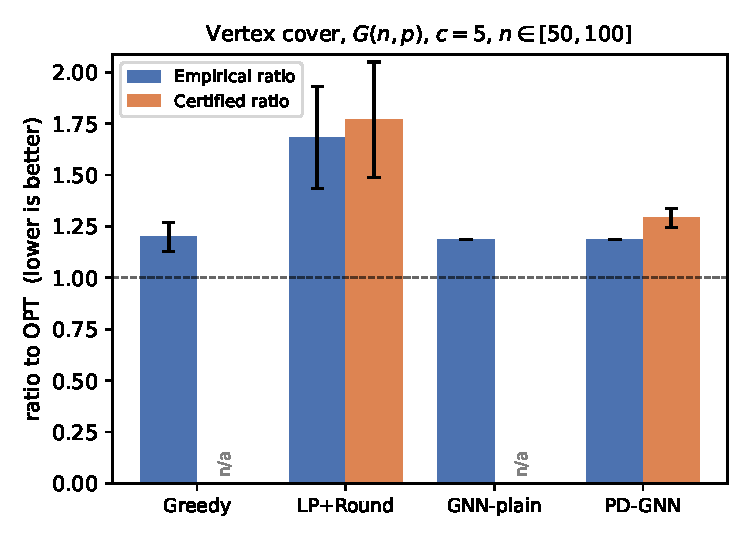
\includegraphics[width=0.48\linewidth]{figures/ratios_er5.pdf}\hfill
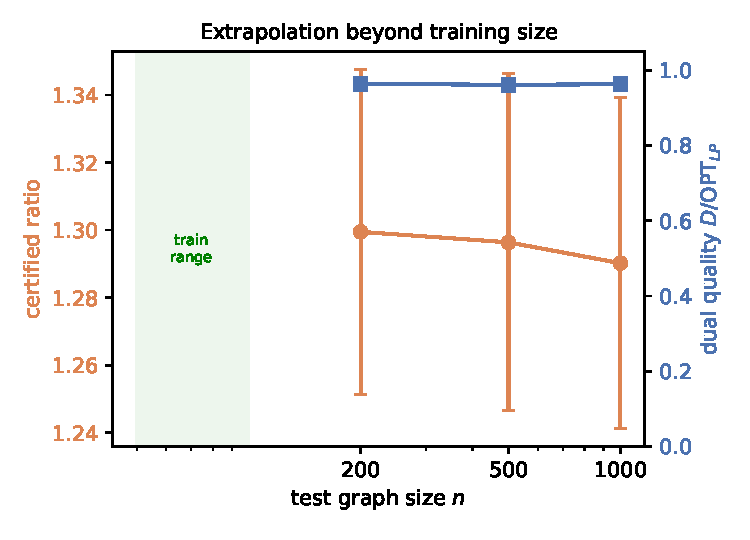
\includegraphics[width=0.48\linewidth]{figures/extrapolation.pdf}
\caption{Left: empirical and certified ratios on $G(n,p)$, $c=5$ (Table~\ref{tab:main}); the certified bar appears only for the two methods that emit a dual. Right: the \PDGNN{} certified ratio and dual quality as the test size grows past the training range.}\label{fig:res}
\end{figure}

\paragraph{Summary.} The experiments confirm the paper's actual claim (Theorem~\ref{thm:cert}): a learned network can emit an always-valid, instance-specific certificate, and with training that certificate is tight. They also surface an honest limitation of the objective rather than the architecture, which Section~\ref{sec:conc} takes up.
